\documentclass{article}


\author{Matthias Maile}
\title{Week 4 Assignment}

\usepackage{amsmath}
\usepackage{graphicx}
\usepackage{float}

% references
\usepackage{hyperref}

\begin{document}
\maketitle
\tableofcontents

\section{Introduction}
\subsection{Typesetting practice}
In \LaTeX, you can write down basically everything you want. For example...
\begin{itemize}
	\item[-] \textbf{Write a bold text,}
	\item[-] write a sharp symbol like \#,
	\item[-] \textsc{or even like this!}
\end{itemize}

\newpage
\subsection{Maxwell`s equations}
\begin{table}[H]
	\begin{tabular}{|c || c | c|}
		\hline
		Name & Integral equations & Differential equations \\
		\hline
		% 1st Gauss law
		Gauss`s law &
		$\oint_{\partial \Omega} \textbf{E} \cdot d\textbf{S} = \frac{1}{\epsilon_0} \int_\Omega \rho dV$ &
		$\nabla \cdot \textbf{E} = \frac{\rho}{\epsilon_o}$ \\
		\hline
		% 2nd Gauss law
		Gauss`s law &
		$\oint_{\partial \Omega} \textbf{B} \cdot d\textbf{S} = 0$ &
		$\nabla \cdot \textbf{B} = 0$ \\
		\hline
		% Faraday law
		Faraday equation &
		$\oint_{\partial \Omega} \textbf{E} \cdot d\textbf{I} = 
		-\frac{d}{dt} \int_{\Sigma} \textbf{B} \cdot d\textbf{S}$ &
		$\nabla \times \textbf{E} = -\frac{\partial\textbf{B}}{\partial t}$ \\
		\hline
		% Amperes Law
		Ampere`s law &
		$\oint_{\partial \Omega} \textbf{B} \cdot d\textbf{I} = 
		\mu_0 \int_{\Sigma} \textbf{J} \cdot d\textbf{S} +
		\mu_0\epsilon_0 \frac{d}{dt} \int_{\Sigma} \textbf{E} \cdot d\textbf{S}$ &
		$\nabla \times \textbf{B} = \mu_0 \left(\textbf{J} + \epsilon_0 \frac{\partial\textbf{E}}{\partial t} \right)$ \\
		\hline
	\end{tabular}
	\caption{4 Maxwell`s equations}
	\label{tab:equations}
\end{table}

\begin{figure}[H]
	\centering
	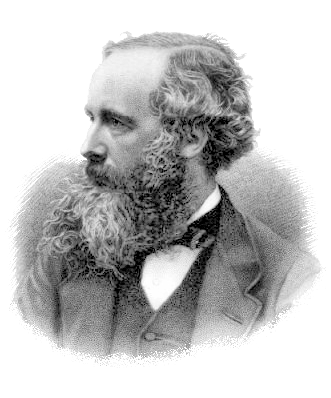
\includegraphics[width=6cm]{James_Clerk_Maxwell.png}
	\caption{James Clerk Maxwell}
	\label{fig:maxwell}
\end{figure}
Maxwell`s equations (\autoref{tab:equations}) is found by J.C.Maxwell (see \autoref{fig:maxwell})

\end{document}
